\documentclass{article}
\usepackage{graphicx} % Required for inserting images
\usepackage[utf8]{inputenc}
\usepackage[french]{babel} %Pour les accents.
\usepackage{amssymb} %Pour les corps.
\usepackage{stmaryrd} %Pour les doubles crochets (intervalles entiers).
\usepackage{enumitem} %Pour énumérer avec autre chose que 1,2,3.
\usepackage{amsmath} %Pour les coefs binomiaux.
\usepackage{float}
\usepackage{array}
\usepackage{listings}
\usepackage[left=2cm,right=2cm,top=2cm,bottom=2cm]{geometry} %Pour régler la taille de la marge.
\usepackage[T1]{fontenc}
\setlength\parindent{0pt}
\usepackage{booktabs}
\usepackage{float}
\usepackage{hyperref}
\hypersetup{
    colorlinks=true,
    linkcolor=blue,
    filecolor=magenta,      
    urlcolor=cyan,
}
\usepackage{easytable}
\usepackage{adjustbox}
\usepackage{tikz,lipsum,lmodern}
\usepackage[most]{tcolorbox}

\newcommand{\bZ}{\mathbb{Z}}

\newcommand{\bun}{\mathbf{1}}
\newcommand{\bN}{\mathbb{N}}
\newcommand{\bR}{\mathbb{R}}
\newcommand{\bP}{\mathbb{P}}
\newcommand{\bE}{\mathbb{E}}
\newcommand{\bV}{\mathbb{V}}
\newcommand{\intbrac}[2]{\llbracket #1,#2\rrbracket}
\newcommand{\Prin}{\operatorname{Prin}}
\newcommand{\Pic}{\operatorname{Pic}}
\newcommand{\deg}{\operatorname{deg}}
\newcommand{\Diag}{\operatorname{Diag}}
\usepackage[backend=biber]{biblatex}
\addbibresource{ref.bib}

\usepackage{fancyhdr}
\usepackage{setspace}
\usepackage{lastpage}

\newcommand{\HRule}{\rule{\linewidth}{0.5mm}}

\pagestyle{fancy}
\renewcommand\headrulewidth{1pt}
\renewcommand\footrulewidth{1pt}
\geometry{headsep=1.1cm}

\fancyhead[L]{
\includegraphics[width=0.1\columnwidth]{./logo}~}
\fancyfoot[L]{\textsc{Algèbre \& Cryptologie
}}
\fancyhead[R]{\textsc{Challenge 1}}
\fancyfoot[C]{\thepage/\pageref{LastPage}}
\fancyfoot[R]{\textsc{\today}}

\title{Algèbre \& Cryptologie : Challenge 1}
\author{Raphaël PAIN DIT HERMIER\\
Alexis LOMBARD-GAILLARD\\
Edward LUCYSZYN}
\date{Avril 2024}

\begin{document}

\begin{titlepage}
\begin{center}

% Upper part of the page. The '~' is needed because only works if a paragraph has started.

\LARGE \textsc{2EL1740: Algèbre \& Cryptologie}

\vspace{0.2cm}

\Large \textsc{CentraleSupélec - 2A}

\vspace{0.3cm}

% Title
\HRule \\[0.4cm]

{\huge \bfseries Challenge 4\\
[0.2cm]}

\HRule \\[0.4cm]

\vspace{2cm}

\textsc{\today}

\vspace{2cm}


\includegraphics[width=0.4\columnwidth]{./logo}~\\[3cm]

% Author and supervisor
\begin{minipage}{0.4\textwidth}
\begin{spacing}{1.125}
\begin{center}
    Raphaël \testsc{PAIN DIT HERMIER}\\
    Alexis \testsc{LOMBARD-GAILLARD}\\
    Edward \testsc{LUCYSZYN}
\end{center}
\end{spacing}
\end{minipage}

\vfill

\end{center}
\end{titlepage}

\tableofcontents

\newpage
\section{Question 1}

\subsection{Conditions de départ, graphe de départ}

Premièrement, on rappelle que l'on considère le graphe $G_7$ constitué des points $\{0,\dots,6\}$, avec un lien entre deux points
$a$ et $b$ si et seulement si $a\neq b$ et $a-b$ est un carré modulo $7$ (i.e. $\exists m \in \bN, a-b\equiv m^2 [7]$).\\
On en déduit que deux points $a,b\in \{0,\dots,6\}$ sont reliés entre eux si $a-b \equiv 1 [7]$ ou $a-b \equiv 2 [7]$ ou $a-b \equiv 4 [7]$.\\

D'après la description donnée par l'énoncé, $G_7$ est un graphe qui relie directement (c'est-à-dire par un seul trait) tous les points entre eux, car pour n'importe quels $a,b\in \{0,\dots,6\}$ tels que $a\neq b$, on a forcément $a-b$ ou $b-a$ qui est un carré modulo 7 (si $a-b$ modulo $7$ vaut $3$, $5$ ou $6$, alors $b-a$ modulo 7 vaudra respectivement $4$, $2$ ou $1$). Donc cette condition n'apporte aucune restriction supplémentaire sur le graphe non orienté. Voici alors un dessin du graphe $G_7$:

\begin{center}
\begin{tikzpicture}

    
    \draw[very thick] (3,6) -- (5.345493,4.87047) -- (5.92479, 2.332437) -- (4.30164, 0.2970933) -- (1.698348, 0.2970933) -- (0.0752163, 2.332437) -- (0.654507, 4.87047) -- (3,6) -- (5.92479, 2.332437) -- (1.698348, 0.2970933) -- (0.654507, 4.87047) -- (5.345493,4.87047) -- (4.30164, 0.2970933) -- (0.0752163, 2.332437) -- (3,6) -- (4.30164, 0.2970933) -- (0.654507, 4.87047) -- (5.92479, 2.332437) -- (0.0752163, 2.332437) -- (5.345493,4.87047) -- (1.698348, 0.2970933) -- (3,6)

    \filldraw  (3,6) circle (3pt)
    \filldraw  (5.345493,4.87047) circle (3pt)
    \filldraw  (5.92479, 2.332437) circle (3pt)
    \filldraw  (4.30164, 0.2970933) circle (3pt)
    \filldraw (1.698348, 0.2970933) circle (3pt)
    \filldraw  (0.0752163, 2.332437) circle (3pt)
    \filldraw  (0.654507, 4.87047) circle (3pt)
    \draw (3,3) node {$G_7$}
    \draw (3,6) node[above]  {$0$}
    \draw (5.345493,4.87047) node[right]  {$1$}
    \draw (5.92479, 2.332437) node[right]  {$2$}
    \draw (4.30164, 0.2970933) node[below]  {$3$}
    \draw (1.698348, 0.2970933) node[below]  {$4$}
    \draw (0.0752163, 2.332437) node[left]  {$5$}
    \draw (0.654507, 4.87047) node[left]  {$6$}
    

\end{tikzpicture}
\end{center}

Avec la convention que le $i$-ème point est $P_i = i-1$, le laplacien de ce graphe est alors $L_{G_7} = (l_{ij})_{1\leq i,j\leq 7}$ où
\[\forall i,j\in \{1,\dots,7\}, l_{ij} = \begin{cases}
    -6 & \textbf{si } i=j;\\
    1 & \textbf{si } i\neq j.
\end{cases}\]

C'est-à-dire

\[L_{G_7} = \begin{pmatrix}
-6&1&1&1&1&1&1\\
1&-6&1&1&1&1&1\\
1&1&-6&1&1&1&1\\
1&1&1&-6&1&1&1\\
1&1&1&1&-6&1&1\\
1&1&1&1&1&-6&1\\
1&1&1&1&1&1&-6\\
\end{pmatrix}\]

On remarquera directement que la matrice est de rang $6$ (possède $0$ comme valeur propre avec le vecteur propre $X = (1,...,1)^\top$), qui apparaîtra donc dans les coefficients diagonaux de sa forme normale de Smith. (c'est en fait le cas pour le laplacien de n'importe quel graphe connexe)\\
On peut calculer la forme normale de Smith du laplacien en implémentant l'algorithme discuté dans \cite{2} sur Python :
\[L_{G_7} = P\Delta Q\]
où
\[\Delta = \Diag(1,7,7,7,7,7,0)\]
et
\[P = \begin{pmatrix} 0&0&0&0&0&0&1\\
0&-1&0&0&0&0&1\\
0&1&-1&0&0&0&0\\
0&0&1&-1&0&0&0\\
0&0&0&1&-1&0&0\\
0&0&0&0&1&-1&0\\
1&1&1&1&1&1&1
\end{pmatrix} ; Q = \begin{pmatrix} 1&-5&-4&-3&-2&-1&-1\\
0&1&0&0&0&0&-1\\
0&1&1&0&0&0&-1\\
0&1&1&1&0&0&-1\\
0&1&1&1&1&0&-1\\
0&1&1&1&1&1&-1\\
0&0&0&0&0&0&-1\end{pmatrix}. \]

On en déduit que ses facteurs invariants sont $(1,7,7,7,7,7,0)$ et donc d'après un corollaire du théorème de Smith :
\[\Pic(G_7) = \mathbb{Z} \times (\mathbb{Z}/7\mathbb{Z})^5.\]

Enfin, son diviseur canonique étant \[K = \sum_{P\in G_7}(|v(P)|-2)(P) = \sum_{P\in G_7}4(P)\]
on en déduit son genre $\displaystyle g = \frac{\deg K}{2}+1 = 15$.\\

\subsection{Conditions de départ, graphe dual}

On rappelle que $G_7^\vee$ est le graphe dual de $G_7$ constitué des mêmes points, avec $a,b$ étant reliés si et seulement si $a,b$ ne sont pas reliés dans $G_7$ (et on rajoutera la condition que $a\neq b$). On dessine maintenant ce graphe $G_7^\vee$:


\begin{center}
\begin{tikzpicture}


    \filldraw  (3,6) circle (3pt)
    \filldraw  (5.345493,4.87047) circle (3pt)
    \filldraw  (5.92479, 2.332437) circle (3pt)
    \filldraw  (4.30164, 0.2970933) circle (3pt)
    \filldraw (1.698348, 0.2970933) circle (3pt)
    \filldraw  (0.0752163, 2.332437) circle (3pt)
    \filldraw  (0.654507, 4.87047) circle (3pt)
    \draw (3,3) node {$G_7^\vee$}
    \draw (3,6) node[above]  {$0$}
    \draw (5.345493,4.87047) node[right]  {$1$}
    \draw (5.92479, 2.332437) node[right]  {$2$}
    \draw (4.30164, 0.2970933) node[below]  {$3$}
    \draw (1.698348, 0.2970933) node[below]  {$4$}
    \draw (0.0752163, 2.332437) node[left]  {$5$}
    \draw (0.654507, 4.87047) node[left]  {$6$}
    

\end{tikzpicture}
\end{center}

On remarque immédiatemment que ce graphe n'est pas connexe, même que chaque point est entièrement isolé. Cependant, rien n'oblige notre étude à se restreindre uniquement à des graphes connexes. On peut en effet voir n'importe quel graphe comme l'union disjointe de plusieurs graphes connexes, et le jeu et les notions vues en cours peuvent s'étendre à n'importe quel graphe.\\
Ceci nous facilite la tâche, car alors $\Prin(G_7^\vee) = \{0\}$ (toute action revient à ne rien faire) et donc $\Pic(G_7^\vee) = \mathbb{Z}^7$.

Enfin, son diviseur canonique étant \[K = \sum_{P\in G_7^\vee}(|v(P)|-2)(P) = \sum_{P\in G_7^\vee}-2(P)\]
on en déduit son genre $\displaystyle g = \frac{\deg K}{2}+1 = -6$.\\

N.B : Dans un cas général, lorsque l'on dispose d'une réunion disjointe de plusieurs graphes $\displaystyle \Gamma = \bigsqcup_{i=1}^n\Gamma_i$, alors on obtient facilement son groupe de Picard $\Pic(\Gamma) = \Pic(\Gamma_1)\times ... \times \Pic(\Gamma_n).$\\

\subsection{Conditions modifiées, graphe de départ}

Tout cela étant dit, nous pourrions penser que la condition sur $G_7$ que "$a-b$ est un carré modulo $7$" aurait plus de sens si elle était couplée avec la condition "$a>b$". Par curiosité, nous allons alors refaire la question avec cette nouvelle condition. On présente le nouveau graphe de $G_7$:

\begin{center}
\begin{tikzpicture}

    
    \draw[very thick] (3,6) -- (5.345493,4.87047) -- (5.92479, 2.332437) -- (4.30164, 0.2970933) -- (1.698348, 0.2970933) -- (0.0752163, 2.332437) -- (0.654507, 4.87047)
    
    \draw[very thick] (3,6) -- (5.92479, 2.332437) -- (1.698348, 0.2970933) -- (0.654507, 4.87047)

    \draw[very thick] (5.345493,4.87047) -- (4.30164, 0.2970933) -- (0.0752163, 2.332437)

    \draw[very thick] (3,6) -- (1.698348, 0.2970933)
    \draw[very thick] (5.345493,4.87047) -- (0.0752163, 2.332437)
    \draw[very thick] (5.92479, 2.332437) -- (0.654507, 4.87047)


    \filldraw  (3,6) circle (3pt)
    \filldraw  (5.345493,4.87047) circle (3pt)
    \filldraw  (5.92479, 2.332437) circle (3pt)
    \filldraw  (4.30164, 0.2970933) circle (3pt)
    \filldraw (1.698348, 0.2970933) circle (3pt)
    \filldraw  (0.0752163, 2.332437) circle (3pt)
    \filldraw  (0.654507, 4.87047) circle (3pt)
    \draw (3,3) node {$G_7$}
    \draw (3,6) node[above]  {$0$}
    \draw (5.345493,4.87047) node[right]  {$1$}
    \draw (5.92479, 2.332437) node[right]  {$2$}
    \draw (4.30164, 0.2970933) node[below]  {$3$}
    \draw (1.698348, 0.2970933) node[below]  {$4$}
    \draw (0.0752163, 2.332437) node[left]  {$5$}
    \draw (0.654507, 4.87047) node[left]  {$6$}



\end{tikzpicture}
\end{center}

Avec la convention que le $i$-ème point est $P_i = i-1$, le laplacien de ce graphe est alors :
\[L_{G_7} = \begin{pmatrix}
-3&1&1&0&1&0&0\\
1&-4&1&1&0&1&0\\
1&1&-5&1&1&0&1\\
0&1&1&-4&1&1&0\\
1&0&1&1&-5&1&1\\
0&1&0&1&1&-4&1\\
0&0&1&0&1&1&-3
\end{pmatrix}\]

On peut calculer la forme normale de Smith du laplacien avec le même algorithme susmentionné :
\[L_{G_7} = P\Delta Q\]
où s'intéressera uniquement à
\[\Delta = \Diag(1,1,1,1,1,1053,0)\]
qui nous donne les facteurs invariants $(1,1,1,1,1,1053,0)$. on en déduit donc que
\[\Pic(G_7) = \bZ\times \bZ/1053\bZ.\]

Son diviseur canonique étant \[K = \sum_{P\in G_7^\vee}(|v(P)|-2)(P) = 1(0) + 2(1) + 3(2) + 2(3) + 3(4) + 2(5) + 1(6)\]
on en déduit son genre $\displaystyle g = \frac{\deg K}{2}+1 = 8$.\\

\subsection{Conditions modifiées, graphe dual}

On dessine maintenant le graphe dual de $G_7$, noté $G_7^\vee$:


\begin{center}
\begin{tikzpicture}


    \draw[very thick] (5.92479, 2.332437) -- (0.0752163, 2.332437) -- (3,6) -- (4.30164, 0.2970933) -- (0.654507, 4.87047) -- (5.345493,4.87047) -- (1.698348, 0.2970933)
    \draw[very thick] (0.654507, 4.87047) -- (3,6)

    \filldraw  (3,6) circle (3pt)
    \filldraw  (5.345493,4.87047) circle (3pt)
    \filldraw  (5.92479, 2.332437) circle (3pt)
    \filldraw  (4.30164, 0.2970933) circle (3pt)
    \filldraw (1.698348, 0.2970933) circle (3pt)
    \filldraw  (0.0752163, 2.332437) circle (3pt)
    \filldraw  (0.654507, 4.87047) circle (3pt)
    \draw (3,3) node {$G_7^\vee$}
    \draw (3,6) node[above]  {$0$}
    \draw (5.345493,4.87047) node[right]  {$1$}
    \draw (5.92479, 2.332437) node[right]  {$2$}
    \draw (4.30164, 0.2970933) node[below]  {$3$}
    \draw (1.698348, 0.2970933) node[below]  {$4$}
    \draw (0.0752163, 2.332437) node[left]  {$5$}
    \draw (0.654507, 4.87047) node[left]  {$6$}
    

\end{tikzpicture}
\end{center}

Le laplacien de ce graphe est alors :
\[L_{G_7^\vee} = \begin{pmatrix}
-3&0&0&1&0&1&1\\
0&-2&0&0&1&0&1\\
0&0&-1&0&0&1&0\\
1&0&0&-2&0&0&1\\
0&1&0&0&-1&0&0\\
1&0&1&0&0&-2&0\\
1&1&0&1&0&0&-3\\
\end{pmatrix}\]

On peut calculer la forme normale de Smith du laplacien :
\[L_{G_7^\vee} = P^\vee\Delta^\vee Q^\vee\]
où s'intéressera uniquement à
\[\Delta^\vee = \Diag(1,1,1,1,1,3,0)\]
qui nous donne les facteurs invariants $(1,1,1,1,1,3,0)$. on en déduit donc que
\[\Pic(G_7^\vee) = \bZ\times \bZ/3\bZ.\]

Son diviseur canonique étant \[K^\vee = \sum_{P\in G_7^\vee}(|v(P)|-2)(P) = 1(0) -1(2) -1(4) + 1(6)\]
on en déduit son genre $\displaystyle g^\vee = \frac{\deg K^\vee}{2}+1 = 1$.
\newpage
\subsection{Bonus}
Lors de ce challenge, nous sommes tombés par hasard sur un résultat intéressant que nous proposons de partager et prouver au sein de ce challenge.

\begin{tcolorbox}[colback=red!5!white,colframe=red!75!black,title=Propriété : Genre du dual]
    Soit $\Gamma$ un graphe de cardinal $|\Gamma| = n\in \bN^*$ et de graphe dual $\Gamma^\vee$. On note $g,g^\vee$ leurs genres respectifs. Alors $\displaystyle g + g^\vee = \frac{(n-1)(n-4)}{2}.$
    \tcblower
    \textbf{Preuve :} Pour $P\in \Gamma$, on note $v(P)$ et $v^\vee(P)$ l'ensemble de ses voisins, respectivement dans $\Gamma$ et dans $\Gamma^\vee$. Par définition du graphe dual, $|v(P)| + |v^\vee(P)| = n-1$. Alors en notant $K$ et $K^\vee$ les diviseurs canoniques respectifs, \[\deg K+\deg K^\vee = \sum_{P\in \Gamma}(|v(P)|-2) + \sum_{P\in \Gamma}(|v^\vee(P)|-2) = \sum_{P\in \Gamma}(n-5) = n(n-5).\]
    Ainsi
    \[g+g^\vee = \frac{\deg K+\deg K^\vee}{2}+2 = \frac{n^2-5n+4}{2} = \frac{(n-1)(n-4)}{2}. \hspace{9pt} \square\]
\end{tcolorbox}

Pour $n=7$, on a bien $\displaystyle \frac{(n-1)(n-4)}{2} = 9$, ce qui concorde avec les couples de genres $(g,g^\vee) = (15,-6)$ et $(g,g^\vee) =(8,1)$ dans la formule démontrée ci-dessus.

\newpage



\section{Question 2}

Pour rappel, le deuxième problème à résoudre consiste à trouver un nombre d'ordre de grandeur $2^{4096}$ qui soit premier et tel que, lorsqu'il est affiché comme une image de taille $64\times 64$, forme un emoji.

\subsection{Analyse du problème}

On a déjà une bonne idée de comment procéder pour trouver un tel nombre : il faut d'abord prendre un nombre qui représente un smiley pour ensuite tester s'il est premier (on ne dispose d'aucun algorithme pour qu'une machine sache si un nombre représente un smiley). D'après le théorème de Damgård–Landrock–Pomerance, la probabilité qu'un entier $n \in \llbracket 2^{4095}, 2^{4096} \rrbracket$ pris uniformément au hasard qui passe le test de Miller-Rabin avec un entier $a$ pris uniformément au hasard soit premier est supérieure à $\displaystyle 1 - 2^{24} \cdot 2^{4 - 2 \sqrt{2^{12}}} = 1 - 2^{24 + 4 - 128} = 1 - 2^{-100}.$ Donc, la probabilité qu'un tel entier soit premier en passant 5 fois le test de Miller-Rabin, est supérieure à $1 - 2^{-500}.$\\ \\
De plus intéressons-nous à la fréquence des nombres premiers entre $2^{4095}$ et $2^{4096}$. Comme ces nombres sont très grands, on peut approximer $\pi(n) \approx \frac{n}{ln(n)}$ le nombre de nombres premiers inférieurs à $n$, la proportion de nombre premiers dans $\llbracket 2^{4095}, 2^{4096} \rrbracket$ est environ égale à :

\begin{align}
    \frac{\pi(2^{4096}) - \pi(2^{4095})}{2^{4096} - 2^{4095}} 
    &= \frac{ \frac{2^{4096}}{\ln(2^{4096})} - \frac{2^{4095}}{\ln(2^{4095})}}{2^{4095}} = \frac{1}{\ln(2)}(\frac{1}{2048} - \frac{1}{4095}) = 0,000352.
    \label{freq}
\end{align}

Cette fréquence nous laisse à penser qu'il faudra environ plusieurs milliers d'essais si nous voulons trouver un nombre premier en prenant un nombre au hasard entre $2^{4095}$ et $2^{4096}$.

\subsection{Première idée de résolution}

Les entiers premiers n'étant pas si rares que ça, une première idée serait de dessiner sur l’écran de pixel les contours du smiley, on dessine alors son smiley “à la main” en ajoutant quelques pixels (puissance de 2) pour qu'il se rapproche de l'ordre de grandeur de $2^{4096}$. Cela nous donnera un nombre assez grand, puis on augmente ce nombre de 1 en 1 jusqu’à tomber sur un nombre probablement premier (comme il ne sera pas considérablement plus grand que celui qui sert au smiley, cela va juste ajouter quelques pixels blancs dans un coin de l’image).\\ \\
En effectuant cette stratégie on obtient l'image suivante.

\begin{figure}[H]
    \centering
    
\includegraphics{Smiley_noir.png}
    \caption{Premier essai pour obtenir un nombre premier en forme de smiley}
    \label{fig:enter-label}
\end{figure}

Soit comme attendu le smiley avec quelques pixels en bas à gauche. 
Le nombre obtenu est:\\ \\
193 079 459 702 973 175 441 354 927 790 855 164 886 071 337 109 974 684 136 531 732 222 820 563 948 736 398 036 354 262 097 074 307 768 708 917 933 471 196 934 025 818 411 037 205 518 672 583 105 323 159 696 283 763 078 144 087 635 033 321 374 546 835 643 216 349 770 952 706 575 024 877 892 063 807 757 006 287 106 632 945 668 702 111 879 295 519 726 810 534 721 772 592 242 868 464 085 785 089 612 234 571 647 814 570 319 606 365 066 626 028 126 262 463 524 934 316 996 001 766 391 865 167 910 772 720 823 286 577 943 275 213 621 691 864 568 697 433 726 239 576 832 621 666 133 971 016 238 919 473 260 974 385 464 170 450 008 013 103 579 738 474 029 244 028 348 446 449 590 392 475 311 435 328 135 817 317 846 616 840 017 160 282 880 749 063 008 995 632 586 254 409 499 839 477 136 002 499 749 719 546 562 069 384 505 808 438 281 912 185 314 062 316 043 931 544 210 795 302 202 981 250 190 053 352 193 381 078 127 351 912 862 590 778 719 194 008 707 746 988 745 911 396 288 727 220 472 148 478 810 761 714 727 164 312 388 679 140 404 011 871 941 132 287 833 935 411 718 039 450 429 146 616 151 708 443 831 030 576 202 070 838 494 247 314 784 873.\\ \\
Seulement ce nombre est assez éloigné de l'ordre de grandeur attendu, on pourrait inverser les pixels noirs et blancs et avoir une stratégie similaire, mais cela est assez insatisfaisant d'avoir des pixels de l'image qui soient parasites juste pour rendre le nombre premier. Donc nous avons changé notre stratégie.

\subsection{Deuxième approche}

Déjà, nous avons réalisé qu'il fallait un entier de l'ordre de $2^{4096}$, ce qui implique que le smiley doit avoir des attributs noirs sur un fond blanc. La technique employée ici, sera de générer une bouche et des yeux rectangulaires avec des hauteurs et des largeurs aléatoires, et de regarder ensuite si ces smileys correspondent à des nombres premiers. Grâce à \eqref{freq}, nous savons qu'il nous faudrait plus de $10000$ smileys pour être un peu près sur de tomber sur un nombre probablement premier.\\ \\
Pour générer les smileys, nous avons tout d'abord défini une zone maximale pour les deux yeux et la bouche, afin de ne pas avoir de smileys trop déformés. Les zones définies ont été faites à la main et sont illustrées dans la Figure~\ref{fig:votre_image}.

\begin{figure}[H]
    \centering
    \begin{tikzpicture}
        % Chargement de l'image
        \node[anchor=south west, inner sep=0] (image) at (0,0) {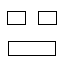
\includegraphics[width=5cm]{zone.png}};
        % Dessin du contour
        \draw[orange,ultra thick] (image.south west) rectangle (image.north east);
    \end{tikzpicture}
    \caption{Zones de limite des yeux et de la bouche}
    \label{fig:votre_image}
\end{figure}

Puis, nous avons codé les fonctions permettant de faire les yeux et la bouche en fonction de la longueur et la hauteur désirées. 

\begin{lstlisting}[language = Python]

def left_eye_pattern_line(height, width, r_max=25, l_max=7, b_max=24, t_max=11):
    matrix = np.zeros((64, 64))

    x_plus = width // 2
    x_minus = - width + x_plus + 1

    y_plus = height//2
    y_minus = - height + y_plus + 1

    for i in range(x_minus, x_plus + 1, 1):
        for j in range(y_minus, y_plus + 1, 1):
            matrix[max(l_max, min(r_max, (r_max + l_max)//2 + i)), \\
            max(t_max, min(b_max, (b_max + t_max)//2 + j))] = 1

    return matrix

def vertical_sym(matrix):
    matrix2 = matrix.copy()
    for x in range(64):
        for y in range(64):
            matrix2[63 - x, y] = matrix[x, y]
    return matrix2

def mouth_pattern_line(height, width, r_max=55, l_max=8, b_max=55, t_max=41):
    matrix = np.zeros((64, 64))

    x_plus = width // 2
    x_minus = - width + x_plus + 1

    y_plus = height//2
    y_minus = - height + y_plus + 1

    for i in range(x_minus, x_plus + 1, 1):
        for j in range(y_minus, y_plus + 1, 1):
            matrix[max(l_max, min(r_max, (r_max + l_max)//2 + i)),\\
            max(t_max, min(b_max, (b_max + t_max)//2 + j))] = 1

    return matrix

\end{lstlisting}

Le code suivant prend bien en compte les bordures des yeux et de la bouche. Une bouche peut avoir $48$ longueurs possibles de ($8$ à $55$) et $15$ hauteurs possibles. Les yeux peuvent avoir $19$ longueurs possibles, et $14$ hauteurs possibles. Cela donne
$48 \cdot 15 \cdot 19^2 \cdot 14^2 = 50 944 302$ smileys différents possibles.\\ \\
Maintenant il faut transformer ces smileys en nombre et leur faire passer le test de Miller-Rabin. 

\begin{lstlisting}[language = Python]
def matrix_coord_to_matrix(matrix):
    matrix2 = np.zeros((64, 64))
    for x in range(64):
        for y in range(64):
            matrix2[63 - y, x] = matrix[x, y]
    return matrix2
    
def create_face(le_height, le_width, m_height, m_width, re_height, re_width):
    return np.ones((64, 64)) - matrix_coord_to_matrix(mouth_pattern_line(m_height, \\
    m_width) + left_eye_pattern_line(le_height, le_width) + \\
    vertical_sym(left_eye_pattern_line(re_height, re_width)))

def matrix_to_number(matrix):
    p = 0
    for i in range(64):
        for j in range(64):
            p += int(matrix[i][j]) * (2**(i*64 + j))
    return p

def create_face_number(le_height, le_width, m_height, m_width, re_height, re_width):
    return matrix_to_number(create_face(le_height, le_width, m_height, \\
    m_width, re_height, re_width))

import random

def miller_rabin_test(n, k=5):
    """
    Test de primalité de Miller-Rabin pour le nombre n.
    Répète le test k fois.
    Retourne True si n est probablement premier, False sinon.
    """
    if n <= 1:
        return False
    if n <= 3:
        return True
    if n % 2 == 0:
        return False
    
    # Écriture de n - 1 comme (2^r * d)
    r, d = 0, n - 1
    while d % 2 == 0:
        r += 1
        d //= 2
    
    # Répéter le test k fois
    for _ in range(k):
        a = random.randint(2, n - 1)
        x = pow(a, d, n)
        if x == 1 or x == n - 1:
            continue
        for _ in range(r - 1):
            x = pow(x, 2, n)
            if x == n - 1:
                break
        else:
            return False
    return True

import time
import os

def main():
    le_height = 1
    le_width = 1
    m_height = 1
    m_width = 1
    re_height = 1
    re_width = 1
    i = 0
    start = time.time()
    while True:
        if miller_rabin_test(create_face_number(le_height, \\
        le_width, m_height, m_width, re_height, re_width)):
            # Save the number in a file in chall1_output
            n = create_face_number(le_height, le_width, m_height, m_width,\\
            re_height, re_width)
            with open(f'chall1_output/{i}_{int(time.time() - start)}.txt', 'w') as f:
                f.write(str(create_face_number(le_height, le_width,\\
                m_height, m_width, \\
                re_height, re_width)))
            # Save the image in a file in chall1_output
            img = Image.new('1', (64, 64)) 
            for k in range(64):
                for j in range(64):
                    img.putpixel((k, 63-j), (n >> (k + (j << 6))) & 1)
            img.save(f'chall1_output/{i}_{int(time.time() - start)}.png')
        le_height = random.randint(1, 14)
        le_width = random.randint(1, 19)
        m_height = random.randint(1, 15)
        m_width = random.randint(1, 48)
        re_height = random.randint(1, 14)
        re_width = random.randint(1, 19)
        i += 1
        # if i % 100 == 0:
        #     print(i, time.time() - start)
\end{lstlisting}

Ce code teste environ $100$ nombres correspondant à des smileys en $30$ secondes (sur nos ordinateurs). Nous sélectionnons les nombres qui passent 5 fois le test de Miller-Rabin.\\ \\
Voici donc une compilation des meilleurs smileys que nous avons eu en faisant tourner le code pendant une nuit.

\begin{figure}[H]
    \centering
    \begin{tikzpicture}
        % Définition de la taille des images et de l'espace entre elles
        \def\imgsize{3cm}
        \def\gap{0.5cm}
        % Boucle pour inclure les images et dessiner les contours rouges
        \foreach \i in {1,...,30} {
            \pgfmathtruncatemacro{\row}{(\i-1)/5}
            \pgfmathtruncatemacro{\col}{(\i-1) - \row*5}
            \node[anchor=south west,inner sep=0] (image\i) at (\col*\imgsize+\col*\gap,-\row*\imgsize-\row*\gap) {\includegraphics[width=\imgsize]{\i.png}};
            \draw[red,ultra thick] (image\i.south west) rectangle (image\i.north east);
        }
    \end{tikzpicture}
    \caption{Exemples de nombres, en forme de smiley, probablement premiers et véritablement premiers avec une probabilité supérieure à $1 - 2^{-500}$.}
    \label{fig:images}
\end{figure}

Par exemple, ici le 16ème correspond au nombre:\\ \\
104 438 888 141 315 250 669 175 271 071 662 438 257 996 424 904 738 378 038 423 348 328 395 390 797 155 745 684 882 681 193 499 755 834 089 010 671 443 926 283 798 757 343 818 579 360 726 323 608 785 136 527 794 595 697 654 370 999 834 036 159 013 438 371 831 442 807 001 185 594 622 637 631 883 939 771 274 567 229 490 868 900 947 883 812 300 526 527 821 791 320 806 926 347 972 397 469 749 073 176 100 249 652 098 019 120 231 115 240 708 302 161 603 094 621 815 668 028 838 318 454 101 231 152 407 083 021 616 030 946 218 156 680 288 383 184 541 014 406 253 539 841 507 323 427 127 013 913 956 594 294 832 799 465 421 168 738 734 067 274 867 731 666 069 282 530 024 068 438 595 393 990 775 495 729 541 288 932 762 687 850 004 496 406 288 597 447 705 636 416 483 473 651 269 221 331 001 440 454 764 427 420 288 503 149 130 420 519 224 955 129 156 490 902 762 725 991 112 521 879 901 668 611 887 283 565 194 084 919 800 377 483 870 548 533 078 094 919 978 378 527 766 189 690 723 160 646 282 124 423 735 272 794 129 263 360 857 519 506 439 951 060 453 729 447 424 537 675 231 883 953 322 051 923 372 969 826 396 928 084 468 130 312 273 839 071 149 908 668 566 255 398 626 506 283 746 696 359 805 142 584 723 309 061 826 647 149 991 867 951 128 102 202 731 354 770 028 077 350 157 721 263 780 699 775 140 345 894 937 588 640 363 303 265 440 333 379 373 918 114 893 526 913 607 843 401 215 875 656 090 720 744 343 025 474 552 544 879 793 901 474 320 368 566 289 139 635 516 689 178 119 018 191 829 967 138 860 343 851 838 261 194 686 309 175 178 555 158 231 714 280 983 587 195 352 990 941 506 066 602 906 265 312 064 094 453 353 726 479 915 058 398 383 008 219 247 078 076 264 032 035 385 601 871 262 515 1.

\newpage

\nocite{*}
\printbibliography

\end{document}
